\documentclass[11pt]{amsart}

\usepackage{mathptmx}
\usepackage{a4wide}
\usepackage{graphicx}

\begin{document}

\section{Classification results}

\begin{center}
  \begin{tabular}[c]{llll}
    \hline
    \texttt{1716.bases}
    & Team Bearland
    & yes
    & 0.33 s
    \\
    & Tresplans
    & yes
    & 0.210 s
    \\
    & Terrible Island
    & yes
    & 121s
    \\
    & A-Team-Has-No-Name
    & yes
    & 28.97 s
    \\
    & other-awesome-team-name
    & yes/no
    & [seconds]
    \\\hline
      \texttt{252.bases}
    & Team Bearland
    & yes
    & 0.007 s
    \\
    & Tresplans
    & yes
    & 0.004 s
    \\
    & Terrible Island
    & yes
    & 0.3 s
    \\
    & A-Team-Has-No-Name
    & yes
    & 0.424 s
    \\\hline
      \texttt{3432.bases}
    & Team Bearland
    & yes
    & 1.276 s
    \\
    & Tresplans
    & yes
    & 0.810 s
    \\
    & A-Team-Has-No-Name
    & yes
    & 131.9 s
    \\\hline
      \texttt{4092.bases}
    & Team Bearland
    & no
    & 0.019 s
    \\
    & Tresplans
    & no
    & 0.001 s
    \\
    & A-Team-Has-No-Name
    & no
    & 2.50 s
    \\\hline
      \texttt{417.bases}
    & Team Bearland
    & no
    & 0.002 s
    \\
    & Tresplans
    & no
    & 0.001 s
    \\
    & Terrible Island
    & no
    & 0.031 s
    \\
    & A-Team-Has-No-Name
    & no
    & 0.151 s
    \\\hline
      \texttt{462.bases}
    & Team Bearland
    & yes
    & 0.021 s
    \\
    & Tresplans
    & yes
    & 0.130 s
    \\
    & Terrible Island
    & yes
    & 2.073 s
    \\
    & A-Team-Has-No-Name
    & yes
    & 1.535 s
    \\\hline
      \texttt{4639.bases}
    & Team Bearland
    & no
    & 0.397 s
    \\
    & Tresplans
    & no
    & 0.001 s
    \\
    & A-Team-Has-No-Name
    & no
    & 3.792 s
    \\\hline
    \texttt{6435.bases}
    & Team Bearland
    & yes
    & 4.506 s
    \\
    & Tresplans
    & yes
    & 2.861 s
    \\
    & A-Team-Has-No-Name
    & yes
    & 508.5 s
    \\\hline
    \texttt{924.bases}
    & Team Bearland
    & yes
    & 0.088 s
    \\
    & Tresplans
    & yes
    & 0.070 s
    \\
    & Terrible Island
    & yes
    & 18.26 s
    \\
    & A-Team-Has-No-Name
    & yes
    & 7.422 s
    \\\hline
    \texttt{definetely-bases.txt}
    & A-Team-Has-No-Name
    & yes
    & 0.00022 s
    \\\hline
    \texttt{not-bases-1.txt}
    & A-Team-Has-No-Name
    & no
    & 0.000282 s
    \\\hline
    \texttt{not-bases-2.txt}
    & A-Team-Has-No-Name
    & no
    & 0.000006 s
    \\\hline    
  \end{tabular}
\end{center}

\section{Execution times}

\subsection{Team Bearland}

We implemented a mask-based algorithm.
Each mask $m$ represents a set.
The $i$-th bit of the mask is set to 1 iff $i$ belongs to the set.
We can easily, and in a fast manner, access each position shifting bits, and unions, intersections and complements are solved using bitwise OR, AND, NOT, and XOR operators.
The code implemented in \textsc{Python3}, albeit leveraging the same principle, implements the masking operations differently.
 
In both cases, the complexity is the same. We take advantage of the fact that all values in all inputs are integers between $0$ and $r - 1 = 19$. In every case, we build the masks in $\mathcal{O}(\sum_{B \in \mathcal{B}} |B|) = \mathcal{O}(r|\mathcal{B}|)$ time. Then, for each pair $(B_1, B_2) \in \mathcal{B} \times \mathcal{B}$, we check that the exchange conditions by taking all $\mathcal{O}(r)$ values of $x \in B_1$, and checking if the condition holds for each of the $\mathcal{O}(r)$ possible values of $y \in B_2$, and we also check that $x \in B_1 \setminus B_2$ and $y \in B_2 \setminus B_1$ in $\mathcal{O}(r^2)$ time. Finally, we check that the mask for $B_1 \setminus \{x\} \cup \{y\}$ belongs to the set of masks in $\mathcal{O}(\log(|\mathcal{B}|))$ time. Therefore, the total complexity is $\mathcal{O}(r |\mathcal{B}|) + \mathcal{O}(r^2 |\mathcal{B}|^2| \log(|\mathcal{B}|)) =  \mathcal{O}(r^2 |\mathcal{B}|^2| \log(|\mathcal{B}|))$.

Figure~\ref{fig:team-bearland-times} summarizes the execution times for both programming languages.
Note that we re-ordered the results to plot them in a, more or less, increasing fashion. 
\begin{figure}[h!]
    \centering
    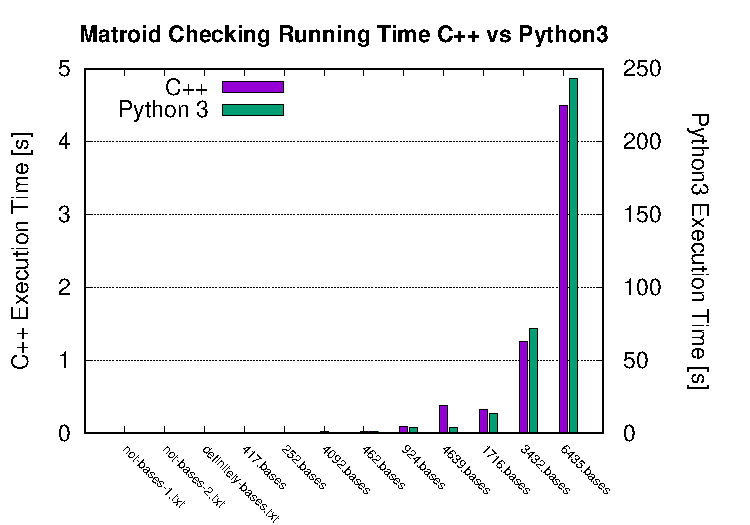
\includegraphics[width=.7\textwidth]{./team-berland/exec_time.pdf}
    \caption{Execution time of the two different implementations in increasing order.\label{fig:team-bearland-times}}
\end{figure}
The results were to be expected, the compiled, performance-oriented, \textsc{C++} implementation outruns the \textsc{Python3} one by two orders of magnitude.
However, we do observe that the behaviour, the pattern described by execution times as we increase the load (\textit{i.e.} the complexity) is the same for both algorithms.
This is a great example not to underestimate the constants affecting our expected running time, usually disregarded by complexity theory and big $\mathcal{O}$ notation.
%Under our point of view, each programming language has it's 

\subsection{Tresplans}

We implemented an algorithm based on hash tables (dictionaries in python).
In order to convert each integer list into a distinct key,
we stored each digit as a shifted bit into a bit array,
the whole list is then the sum of all bits (with an OR operation).
This method gives us distinct keys for each list of integers.
With this method,
we have been able to process all files.

Then, we can check if a list of bases exist in the hash table in a constant time.
The operation
\(x \in B_1 \setminus B_2\)
is implemented as
\(B_1 \land \neg B_2\)
on the bit array and selecting digits on the resulting bit array
(similar for \(y\)).
The operation
\(B_1 \setminus \{x\} \cup \{y\}\)
is also implemented as
\(B_1 \land \neg \{x\} \lor \{y\}\).

The complexity of our code is the same in both implementations.
It can be computed as follows, where $N$ is the number of bases:

\begin{itemize}
 \item Process file: $\mathcal{O}(N)$.
 \item Compare bases: $\mathcal{O}(N^2)$.
 \item Compare each pair of subsets of the base:
       constant time, with a large constant.
\end{itemize}

Thus, overall complexity is $\mathcal{O}(N^2)$.
It is also output-sensitive,
as it stops if it finds a pair of bases do not satisfy the exchange axiom.

In figure~\ref{fig:Tresplans} we have the running time of both implementations.

\begin{figure}[h!]
    \centering
    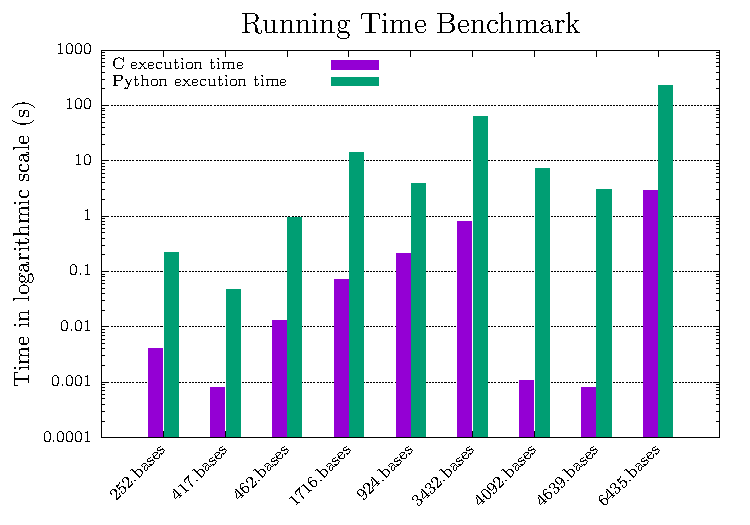
\includegraphics[width=.75\textwidth]{./Tresplans/Tresplans_exec_time.pdf}
    \caption{Execution times of the different implementations.
    \label{fig:Tresplans}}
\end{figure}

Time is displayed in logarithm scale to be able to compare it better,
as the values have a large span either between the same implementations,
and within the same implementation with different files.
Note that as the algorithm is output-sensitive,
a larger file not always leads to larger execution times,
as if there is a pair of bases that do not satisfy the exchange axiom,
then the routine exits.

It is clear that the \textsc{C} implementation is much faster in all cases.
The \textsc{Python} implementation takes a long time to build the dictionary.
It can be observed as the running time is much similar to the
\textsc{C} implementation when the file is large.
Also, most of the difference is because \textsc{Python} checks the type
of the variables in running time,
while in the case of the \textsc{C} code,
it does not happen and mostly works with memory addresses.

In both cases,
due to the complexity of the algorithm
and the fact that in each iteration we need to do a lot of operations and checks,
the execution times grow orders of magnitudes when comparing different files.

\subsection{Terrible Island}
\label{terribleisland}

Both codes follow the same procedure, in that they check, for every base, all other bases, and then in each of these pairs, we check the exchange axiom. If we consider a set of $n$ bases, and $m$ to be the longest check for the exchange axiom (which will be at most the size of the largest base in the set), the complexity of the algorithm is $O(n^{2}m)$.

As it can be seen in \ref{figureterribleisland}, the execution times increase quickly with the number of bases in the files (in the cases they are matroids). Quite unexpectedly, the \textsc{Python} execution times are a lot faster than the \textsc{Julia} ones, the earlier being capable of processing up to 1716 bases before the time limit in contrast to the 924 of the later.

All pairs are checked twice in these algorithms, which could be optimised so the running time would be halved, though this would still keep the complexity at $O(n^{2}m)$.

\begin{figure}[h!]
	\centering
	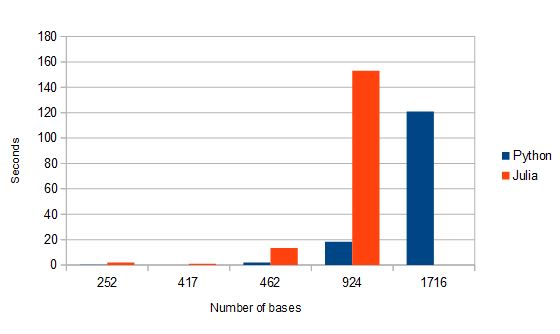
\includegraphics[width=.7\textwidth]{./Terrible-Island/times.jpeg}
	\caption{Execution times of the algorithms \ref{terribleisland}}
	\label{figureterribleisland}
\end{figure}

\subsection{A-team-has-no-name}

1)Our code can process all the files, but the Haskell version takes 11 thousand seconds for the largest file and the python best algorithm takes 917 seconds which is still a lot.

2)If n is the number of elements in $\mathcal{B}$ and m the max number of elements in any of the elements of $\mathcal{B}$, our first python code runs in $\mathcal{O}(n^3)*\mathcal{O}(m^4)$.
We could reduce the complexity concerning m, but as in almost any case we can find m is going to be a constant amount compared to n, we have not worried a lot about it as the complexity for those kinds of general examples is actually $\mathcal{O}(n^3)$.
We tried to reduce this complexity by trying to check relations between the elements in B but at first we ended up making the complexity worse, and then when improved we returned back to $\mathcal{O}(n^3)$ but reducing the running time to a 60\%-70\% of the original one for the files we processed.

Haskell code runs equally in $\mathcal{O}(n^3)$.

For the second python code we thought about using a bijection between sets of integers and integer numbers so that we could order the list of sets and check if $B_1$ is in the list in logarithmic time.
This was done by assigning every set the sum of 2 powered to every of the elements in the set. 
This assumes that we are using integers for each set in the matroid and that there are not a lot of elements in total. If there were other elements that were not integers we could do a bijection between the elements and $\mathbb{Z}$ so we could apply this method.
This allows us to avoid the last loop by using a binary search in the ordered set of values of each element in the matroid, reducing the complexity to $\mathcal{O}(n^3)*\log(n)$. 
If m was big we expect this algorithm to be worse than the first one, so it is input sensitive. 

For the last python code we changed the ordered list by a hash table (sets in Python) so that the search for an element runs in average in $\mathcal{O}(1)$ time instead of $\mathcal{O}(\log(n))$ time.
In general this version is quicker but in the worst possible case it is worse than the previous one.
More exactly this version has an expected complexity of $\mathcal{O}(n^2)$ and a (worst-case) complexity of $\mathcal{O}(n^3)$.

It is also worth mentioning that both of the python algorithms will stop as soon as they find a $B_1$ that does not verify the condition, and that is why 4096.bases files or similar get checked so quickly.

The algorithms are described in the code in form of commentaries.


\subsection{other-awesome-team-name}

another plot here

\end{document}
